\chapter{Experiments and results} \label{sec:experiments-and-results}

Results trying to define a good baseline:
\begin{comment}

\begin{table}[h!]
  \centering
  \begin{tabular}{|c|c|c|c|c|c|c|c|}
    \hline
    & \multicolumn{2}{c|}{\textbf{Method}} & \multicolumn{3}{c|}{\textbf{Metrics}} & \multicolumn{2}{c|}{\textbf{Performance}} \\ \cline{2-8} 
    \textbf{Exp.} & \textbf{Name} & \textbf{Method} & \textbf{PSNR} & \textbf{SSIM} & \textbf{LPIPS} & \textbf{Num Rays per Sec} & \textbf{FPS} \\ 
    \textbf{ID} & & & & & & & \\ \hline
    0 & exp\_image\_size-0 & nerfacto & 23.35 & 0.75 & 0.08 & 389663 & 12.99 \\ \hline
    1 & exp\_image\_size-1 & nerfacto & 23.61 & 0.78 & 0.10 & 458438 & 3.82 \\ \hline
    2 & exp\_image\_size-2 & nerfacto & 23.24 & 0.76 & 0.17 & 494213 & 1.03 \\ \hline
    3 & exp\_image\_size-3 & nerfacto & 23.07 & 0.73 & 0.23 & 513221 & 0.48 \\ \hline
    4 & exp\_image\_size-4 & nerfacto & 22.82 & 0.73 & 0.27 & 522610 & 0.27 \\ \hline
  \end{tabular}
  \caption{Experimental results for different image sizes and rendering methods.}
  \label{tab:exp_results}
\end{table}

\begin{table}[h!]
  \centering
  \begin{tabular}{|c|c|c|c|c|c|c|c|}
    \hline
    & \multicolumn{2}{c|}{\textbf{Method}} & \multicolumn{3}{c|}{\textbf{Metrics}} & \multicolumn{2}{c|}{\textbf{Performance}} \\ \cline{2-8} 
    \textbf{Exp.} & \textbf{Name} & \textbf{Method} & \textbf{PSNR} & \textbf{SSIM} & \textbf{LPIPS} & \textbf{Num Rays per Sec} & \textbf{FPS} \\ 
    \textbf{ID} & & & & & & & \\ \hline
    0 & exp\_speed-0 & nerfacto & 24.06 & 0.78 & 0.18 & 526011 & 1.95 \\ \hline
    1 & exp\_speed-1 & nerfacto & 23.50 & 0.76 & 0.18 & 503773 & 1.87 \\ \hline
    2 & exp\_speed-2 & nerfacto & 23.41 & 0.74 & 0.19 & 504456 & 1.87 \\ \hline
    3 & exp\_speed-3 & nerfacto & 22.72 & 0.71 & 0.20 & 500471 & 1.85 \\ \hline
  \end{tabular}
  \caption{Experimental results for different speed configurations and rendering methods.}
  \label{tab:exp_results}
\end{table}

\begin{table}[h!]
  \centering
  \begin{tabular}{|c|c|c|c|c|c|c|c|}
    \hline
    & \multicolumn{2}{c|}{\textbf{Method}} & \multicolumn{3}{c|}{\textbf{Metrics}} & \multicolumn{2}{c|}{\textbf{Performance}} \\ \cline{2-8} 
    \textbf{Exp.} & \textbf{Name} & \textbf{Method} & \textbf{PSNR} & \textbf{SSIM} & \textbf{LPIPS} & \textbf{Num Rays per Sec} & \textbf{FPS} \\ 
    \textbf{ID} & & & & & & & \\ \hline
    0 & exp\_frames-0 & nerfacto & \cellcolor{green}23.258400 & 0.723872 & 0.228383 & 536168.125000 & 1.985808 \\ \hline
    1 & exp\_frames-1 & nerfacto & 23.251682 & \cellcolor{red}0.727191 & \cellcolor{green}0.221351 & 525303.812500 & 1.945570 \\ \hline
    2 & exp\_frames-2 & nerfacto & 22.557207 & 0.696930 & 0.239964 & 527543.687500 & 1.953866 \\ \hline
    3 & exp\_frames-3 & nerfacto & 22.219042 & 0.685168 & 0.250390 & 518148.062500 & 1.919067 \\ \hline
    4 & exp\_frames-4 & nerfacto & \cellcolor{red}21.917959 & 0.678348 & 0.258932 & 514980.000000 & 1.907333 \\ \hline
  \end{tabular}
  \caption{Experimental results for different frame configurations and rendering methods.}
  \label{tab:exp_results}
\end{table}

I extracted the table data from the HTML and combined it into a single LaTeX table. Here it is:

\begin{table}[ht]
\centering
\begin{tabular}{|c|c|c|c|c|c|c|c|}
\hline
 & \textbf{exp\_name} & \textbf{method\_name} & \textbf{psnr} & \textbf{ssim} & \textbf{lpips} & \textbf{num\_rays\_per\_sec} & \textbf{fps} \\ \hline
0 & exp\_speed-0 & nerfacto & 24.061440 & 0.775393 & 0.181360 & 526011.000000 & 1.948189 \\ \hline
1 & exp\_speed-1 & nerfacto & 23.502066 & 0.755476 & 0.184455 & 503773.000000 & 1.865826 \\ \hline
2 & exp\_speed-2 & nerfacto & 23.411259 & 0.742473 & 0.189968 & 504455.656250 & 1.868354 \\ \hline
3 & exp\_speed-3 & nerfacto & 22.717318 & 0.713858 & 0.200099 & 500470.937500 & 1.853596 \\ \hline
0 & exp\_image\_size-0 & nerfacto & 23.349852 & 0.748548 & 0.081860 & 389662.656250 & 12.988756 \\ \hline
1 & exp\_image\_size-1 & nerfacto & 23.613869 & 0.775704 & 0.103645 & 458438.406250 & 3.820320 \\ \hline
2 & exp\_image\_size-2 & nerfacto & 23.242430 & 0.762787 & 0.168621 & 494213.156250 & 1.029611 \\ \hline
3 & exp\_image\_size-3 & nerfacto & 23.073208 & 0.731756 & 0.232993 & 513221.375000 & 0.475205 \\ \hline
4 & exp\_image\_size-4 & nerfacto & 22.822489 & 0.727354 & 0.267016 & 522609.656250 & 0.272193 \\ \hline
\end{tabular}
\caption{Combined table data}
\label{tab:combined_table}
\end{table}
\begin{table}[ht]
\centering

\begin{tabular}{|c|c|c|c|c|c|c|c|}
\hline
 & \textbf{exp\_name} & \textbf{method\_name} & \textbf{psnr} & \textbf{ssim} & \textbf{lpips} & \textbf{num\_rays\_per\_sec} & \textbf{fps} \\ \hline
0 & exp\_speed-0 & nerfacto & 24.061440 & 0.775393 & 0.181360 & 526011.000000 & 1.948189 \\ \hline
1 & exp\_speed-1 & nerfacto & 23.502066 & 0.755476 & 0.184455 & 503773.000000 & 1.865826 \\ \hline
2 & exp\_speed-2 & nerfacto & 23.411259 & 0.742473 & 0.189968 & 504455.656250 & 1.868354 \\ \hline
3 & exp\_speed-3 & nerfacto & 22.717318 & 0.713858 & 0.200099 & 500470.937500 & 1.853596 \\ \hline
0 & exp\_image\_size-0 & nerfacto & 23.349852 & 0.748548 & 0.081860 & 389662.656250 & 12.988756 \\ \hline
1 & exp\_image\_size-1 & nerfacto & 23.613869 & 0.775704 & 0.103645 & 458438.406250 & 3.820320 \\ \hline
2 & exp\_image\_size-2 & nerfacto & 23.242430 & 0.762787 & 0.168621 & 494213.156250 & 1.029611 \\ \hline
3 & exp\_image\_size-3 & nerfacto & 23.073208 & 0.731756 & 0.232993 & 513221.375000 & 0.475205 \\ \hline
4 & exp\_image\_size-4 & nerfacto & 22.822489 & 0.727354 & 0.267016 & 522609.656250 & 0.272193 \\ \hline
0 & exp\_capacity-0 & nerfacto & 23.541059 & 0.773228 & 0.108571 & 433723.843750 & 1.606385 \\ \hline
1 & exp\_capacity-1 & nerfacto & 23.594120 & 0.763471 & 0.141350 & 479196.437500 & 1.774802 \\ \hline
2 & exp\_capacity-2 & nerfacto & 23.599499 & 0.756889 & 0.181586 & 512589.781250 & 1.898480 \\ \hline
3 & exp\_capacity-3 & nerfacto & 22.634428 & 0.719888 & 0.210503 & 522639.875000 & 1.935703 \\ \hline
4 & exp\_capacity-4 & nerfacto & 22.500532 & 0.695553 & 0.240513 & 527381.250000 & 1.953264 \\ \hline
\end{tabular}
\caption{Expanded table data}
\label{tab:expanded_table}
\end{table}

\begin{table}[ht]
\centering
\begin{tabular}{|c|c|c|c|c|c|c|c|}
\hline
 & \textbf{exp\_name} & \textbf{method\_name} & \textbf{psnr} & \textbf{ssim} & \textbf{lpips} & \textbf{num\_rays\_per\_sec} & \textbf{fps} \\ \hline
0 & exp\_speed-0 & nerfacto & 24.061440 & 0.775393 & 0.181360 & 526011.000000 & 1.948189 \\ \hline
1 & exp\_speed-1 & nerfacto & 23.502066 & 0.755476 & 0.184455 & 503773.000000 & 1.865826 \\ \hline
2 & exp\_speed-2 & nerfacto & 23.411259 & 0.742473 & 0.189968 & 504455.656250 & 1.868354 \\ \hline
3 & exp\_speed-3 & nerfacto & 22.717318 & 0.713858 & 0.200099 & 500470.937500 & 1.853596 \\ \hline
0 & exp\_image\_size-0 & nerfacto & 23.349852 & 0.748548 & 0.081860 & 389662.656250 & 12.988756 \\ \hline
1 & exp\_image\_size-1 & nerfacto & 23.613869 & 0.775704 & 0.103645 & 458438.406250 & 3.820320 \\ \hline
2 & exp\_image\_size-2 & nerfacto & 23.242430 & 0.762787 & 0.168621 & 494213.156250 & 1.029611 \\ \hline
3 & exp\_image\_size-3 & nerfacto & 23.073208 & 0.731756 & 0.232993 & 513221.375000 & 0.475205 \\ \hline
4 & exp\_image\_size-4 & nerfacto & 22.822489 & 0.727354 & 0.267016 & 522609.656250 & 0.272193 \\ \hline
0 & exp\_capacity-0 & nerfacto & 23.541059 & 0.773228 & 0.108571 & 433723.843750 & 1.606385 \\ \hline
1 & exp\_capacity-1 & nerfacto & 23.594120 & 0.763471 & 0.141350 & 479196.437500 & 1.774802 \\ \hline
2 & exp\_capacity-2 & nerfacto & 23.599499 & 0.756889 & 0.181586 & 512589.781250 & 1.898480 \\ \hline
3 & exp\_capacity-3 & nerfacto & 22.634428 & 0.719888 & 0.210503 & 522639.875000 & 1.935703 \\ \hline
4 & exp\_capacity-4 & nerfacto & 22.500532 & 0.695553 & 0.240513 & 527381.250000 & 1.953264 \\ \hline
0 & exp\_camera\_setup-0 & nerfacto & 23.900909 & 0.782013 & 0.135604 & 489572.093750 & 1.813230 \\ \hline
1 & exp\_camera\_setup-1 & nerfacto & 23.235004 & 0.755689 & 0.155470 & 488309.812500 & 1.808555 \\ \hline
2 & exp\_camera\_setup-2 & nerfacto & 23.732924 & 0.739246 & 0.174111 & 492206.968750 & 1.822989 \\ \hline
3 & exp\_camera\_setup-3 & nerfacto & 24.318214 & 0.739551 & 0.172868 & 493037.125000 & 1.826064 \\ \hline
4 & exp\_camera\_setup-4 & nerfacto & 23.785522 & 0.763684 & 0.165152 & 506921.562500 & 1.877487 \\ \hline
5 & exp\_camera\_setup-5 & nerfacto & 23.684502 & 0.754842 & 0.176524 & 506154.500000 & 1.874646 \\ \hline
\end{tabular}
\caption{Expanded table data}
\label{tab:expanded_table}
\end{table}

\begin{table}[ht]
\centering
\begin{tabular}{|c|c|c|c|c|c|c|c|}
\hline
 & \textbf{exp\_name} & \textbf{method\_name} & \textbf{psnr} & \textbf{ssim} & \textbf{lpips} & \textbf{num\_rays\_per\_sec} & \textbf{fps} \\ \hline
0 & exp\_speed-0 & nerfacto & 24.061440 & 0.775393 & 0.181360 & 526011.000000 & 1.948189 \\ \hline
1 & exp\_speed-1 & nerfacto & 23.502066 & 0.755476 & 0.184455 & 503773.000000 & 1.865826 \\ \hline
2 & exp\_speed-2 & nerfacto & 23.411259 & 0.742473 & 0.189968 & 504455.656250 & 1.868354 \\ \hline
3 & exp\_speed-3 & nerfacto & 22.717318 & 0.713858 & 0.200099 & 500470.937500 & 1.853596 \\ \hline
0 & exp\_image\_size-0 & nerfacto & 23.349852 & 0.748548 & 0.081860 & 389662.656250 & 12.988756 \\ \hline
1 & exp\_image\_size-1 & nerfacto & 23.613869 & 0.775704 & 0.103645 & 458438.406250 & 3.820320 \\ \hline
2 & exp\_image\_size-2 & nerfacto & 23.242430 & 0.762787 & 0.168621 & 494213.156250 & 1.029611 \\ \hline
3 & exp\_image\_size-3 & nerfacto & 23.073208 & 0.731756 & 0.232993 & 513221.375000 & 0.475205 \\ \hline
4 & exp\_image\_size-4 & nerfacto & 22.822489 & 0.727354 & 0.267016 & 522609.656250 & 0.272193 \\ \hline
0 & exp\_capacity-0 & nerfacto & 23.541059 & 0.773228 & 0.108571 & 433723.843750 & 1.606385 \\ \hline
1 & exp\_capacity-1 & nerfacto & 23.594120 & 0.763471 & 0.141350 & 479196.437500 & 1.774802 \\ \hline
2 & exp\_capacity-2 & nerfacto & 23.599499 & 0.756889 & 0.181586 & 512589.781250 & 1.898480 \\ \hline
3 & exp\_capacity-3 & nerfacto & 22.634428 & 0.719888 & 0.210503 & 522639.875000 & 1.935703 \\ \hline
4 & exp\_capacity-4 & nerfacto & 22.500532 & 0.695553 & 0.240513 & 527381.250000 & 1.953264 \\ \hline
0 & exp\_camera\_setup-0 & nerfacto & 23.900909 & 0.782013 & 0.135604 & 489572.093750 & 1.813230 \\ \hline
1 & exp\_camera\_setup-1 & nerfacto & 23.235004 & 0.755689 & 0.155470 & 488309.812500 & 1.808555 \\ \hline
2 & exp\_camera\_setup-2 & nerfacto & 23.732924 & 0.739246 & 0.174111 & 492206.968750 & 1.822989 \\ \hline
3 & exp\_camera\_setup-3 & nerfacto & 24.318214 & 0.739551 & 0.172868 & 493037.125000 & 1.826064 \\ \hline
4 & exp\_camera\_setup-4 & nerfacto & 23.785522 & 0.763684 & 0.165152 & 506921.562500 & 1.877487 \\ \hline
5 & exp\_camera\_setup-5 & nerfacto & 23.684502 & 0.754842 & 0.176524 & 506154.500000 & 1.874646 \\ \hline
0 & exp\_frames-0 & nerfacto & 23.258400 & 0.723872 & 0.228383 & 536168.125000 & 1.985808 \\ \hline
1 & exp\_frames-1 & nerfacto & 23.251682 & 0.727191 & 0.221351 & 525303.812500 & 1.945570 \\ \hline
2 & exp\_frames-2 & nerfacto & 22.557207 & 0.696930 & 0.239964 & 527543.687500 & 1.953866 \\ \hline
3 & exp\_frames-3 & nerfacto & 22.219042 & 0.685168 & 0.250390 & 518148.062500 & 1.919067 \\ \hline
4 & exp\_frames-4 & nerfacto & 21.917959 & 0.678348 & 0.258932 & 514980.000000 & 1.907333 \\ \hline
\end{tabular}
\caption{Expanded table data}
\label{tab:expanded_table}
\end{table}

\begin{table}[ht]
\centering
\begin{tabular}{|c|c|c|c|c|}
\hline
 & \textbf{exp\_name} & \textbf{psnr} & \textbf{ssim} & \textbf{lpips} \\ \hline
0 & exp\_speed-0 & 24.061440 & 0.775393 & 0.181360 \\ \hline
1 & exp\_speed-1 & 23.502066 & 0.755476 & 0.184455 \\ \hline
2 & exp\_speed-2 & 23.411259 & 0.742473 & 0.189968 \\ \hline
3 & exp\_speed-3 & 22.717318 & 0.713858 & 0.200099 \\ \hline
0 & exp\_image\_size-0 & 23.349852 & 0.748548 & 0.081860 \\ \hline
1 & exp\_image\_size-1 & 23.613869 & 0.775704 & 0.103645 \\ \hline
2 & exp\_image\_size-2 & 23.242430 & 0.762787 & 0.168621 \\ \hline
3 & exp\_image\_size-3 & 23.073208 & 0.731756 & 0.232993 \\ \hline
4 & exp\_image\_size-4 & 22.822489 & 0.727354 & 0.267016 \\ \hline
0 & exp\_capacity-0 & 23.541059 & 0.773228 & 0.108571 \\ \hline
1 & exp\_capacity-1 & 23.594120 & 0.763471 & 0.141350 \\ \hline
2 & exp\_capacity-2 & 23.599499 & 0.756889 & 0.181586 \\ \hline
3 & exp\_capacity-3 & 22.634428 & 0.719888 & 0.210503 \\ \hline
4 & exp\_capacity-4 & 22.500532 & 0.695553 & 0.240513 \\ \hline
0 & exp\_camera\_setup-0 & 23.900909 & 0.782013 & 0.135604 \\ \hline
1 & exp\_camera\_setup-1 & 23.235004 & 0.755689 & 0.155470 \\ \hline
2 & exp\_camera\_setup-2 & 23.732924 & 0.739246 & 0.174111 \\ \hline
3 & exp\_camera\_setup-3 & 24.318214 & 0.739551 & 0.172868 \\ \hline
4 & exp\_camera\_setup-4 & 23.785522 & 0.763684 & 0.165152 \\ \hline
5 & exp\_camera\_setup-5 & 23.684502 & 0.754842 & 0.176524 \\ \hline
0 & exp\_frames-0 & 23.258400 & 0.723872 & 0.228383 \\ \hline
1 & exp\_frames-1 & 23.251682 & 0.727191 & 0.221351 \\ \hline
2 & exp\_frames-2 & 22.557207 & 0.696930 & 0.239964 \\ \hline
3 & exp\_frames-3 & 22.219042 & 0.685168 & 0.250390 \\ \hline
4 & exp\_frames-4 & 21.917959 & 0.678348 & 0.258932 \\ \hline
\end{tabular}
\caption{Updated table data without num\_rays\_per\_sec, fps, and method\_name columns}
\label{tab:updated_table}
\end{table}

\begin{table}
\centering
\caption{Results for exp_speed-2}
\label{tab:exp_speed-2}
\begin{tabular}{|l|c|c|c|c|}
\toprule
 & description & psnr & ssim & lpips \\
\midrule
0 & 0 & {\cellcolor{green}} 24.061440 & {\cellcolor{green}} 0.775393 & {\cellcolor{red}} 0.181360 \\
\cline{1-5}
1 & 1 & 23.502066 & 0.755476 & 0.184455 \\
\cline{1-5}
2 & 2 & 23.411259 & 0.742473 & 0.189968 \\
\cline{1-5}
3 & 3 & {\cellcolor{red}} 22.717318 & {\cellcolor{red}} 0.713858 & {\cellcolor{green}} 0.200099 \\
\cline{1-5}
\bottomrule
\end{tabular}
\end{table}

\end{comment}

\section{Defining a baseline}

In order to do multiple experiments I needed a baseline to compare subsequent experiments with. There aren't any baselines on NeRFs with data gathered from CARLA, so I made my own.

The baseline is put together by combining the best setup from the following categories:

CARLA:
\begin{itemize}
    \item Camera-setup
    \item Capacity
    \item Camera settings (image size)
    \item Vehicle speed
    \item Number of frames
\end{itemize}

NeRF:
\begin{itemize}
    \item Model
    \item Camera optimization
\end{itemize}

\subsection{Camera setup}
In the CARLA simulator you can easily attach multiple cameras with different settings to the vehicle. NeRF operates on RGB-images, so I chose to experiment with which camera setups yielded the best results over the three metrics, PSNR, SSIM and LPIPS.

The camera setups I tested were:
\begin{itemize}
    \item Single forward-facing camera
    \item Two forward-facing cameras, with a counterrotated yaw
    \item Three cameras, one with zero yaw and two with yaw
\end{itemize}

\begin{table}[ht]
\centering
\begin{tabular}{|l|c|c|c|c|}
\hline
& description & psnr & ssim & lpips \\
\hline
10 & 10 & 22.764567 & 0.74230 & 0.150325 \\
\cline{1-5}
\textbf{0} & 0 & 23.900909 & $\cellcolor{green} 0.782013$ & $\cellcolor{green} 0.135604$ \\
\cline{1-5}
1 & 1 & $\cellcolor{red} 23.235004$ & 0.755689 & 0.155470 \\
\cline{1-5}
2 & 2 & 23.732924 & $\cellcolor{red} 0.739246$ & 0.174111 \\
\cline{1-5}
3 & 3 & $\cellcolor{green} 24.318214$ & 0.739551 & 0.172868 \\
\cline{1-5}
4 & 4 & 23.785522 & 0.763684 & 0.165152 \\
\cline{1-5}
5 & 5 & 23.684502 & 0.754842 & $\cellcolor{red} 0.176524$ \\
\cline{1-5}
\end{tabular}
\caption{Results for exp\_camera\_setup-5}
\label{tab:exp_camera_setup-5}
\end{table}

% ADD THIS TO THE DISCUSSION-PART
From the table we see that there's not that much different across the metrics. Setup 3 with two cameras pointing with $-70^\circ$ and $70^\circ$ yaw achieves the best PSNR. Setup 1 does best on SSIM and LPIPS and achieves the second best PSNR.

Setup 0 eller 3
- 0 har bedre SSIM og LPIPS, og nesten like god PSNR.

\subsection{Capacity}
Scaling NeRFs to larger scenes isn’t trivial. The underlying MLP only has a certain capacity, and if we were to increase the capacity, training times would increase and rendering times would scale linearly. Rendering is already an expensive operation which further supports the claim for another solution. But, what is the capacity of a NeRF?

In order to try and answer this I created 5 increasingly longer routes for the CARLA-vehicle to gather data on, from 50m to ~450m. The route that's ~450m long is equivalent to one full lap around the block.

\begin{table}[ht]
\centering
\begin{tabular}{|l|c|c|c|c|}
\hline
  & description & psnr & ssim & lpips \\
\hline
0 & 0 & 23.541059 & $\cellcolor{green} 0.773228$ & $\cellcolor{green} 0.108571$ \\
\cline{1-5}
1 & 1 & 23.594120 & 0.763471 & 0.141350 \\
\cline{1-5}
2 & 2 & $\cellcolor{green} 23.599499$ & 0.756889 & 0.181586 \\
\cline{1-5}
3 & 3 & 22.634428 & 0.719888 & 0.210503 \\
\cline{1-5}
4 & 4 & $\cellcolor{red} 22.500532$ & $\cellcolor{red} 0.695553$ & $\cellcolor{red} 0.240513$ \\
\cline{1-5}
\end{tabular}
\caption{Results for exp\_capacity-2}
\label{tab:exp_capacity-2}
\end{table}

% ADD THIS TO THE DISCUSSION-PART
As expected, the results degrade as the segments' length increases.

\begin{figure}[!h]
    \centering
    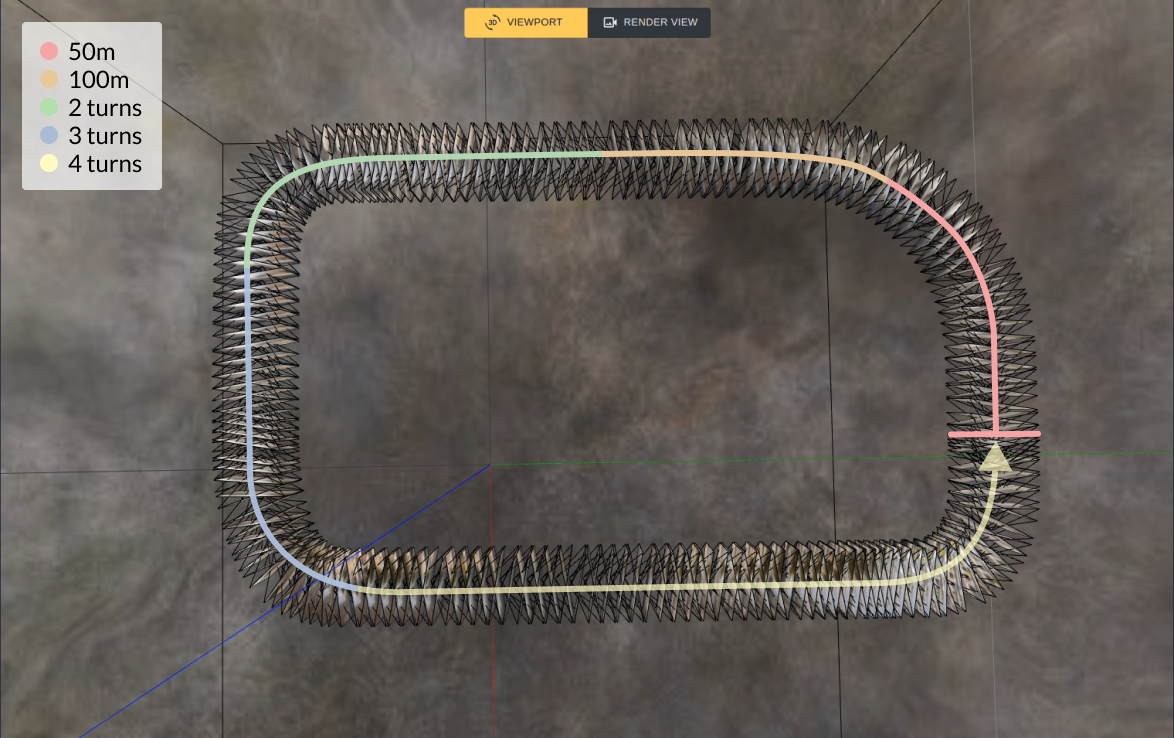
\includegraphics[width=1.0\textwidth]{figures/capacity-overview.png}
    \caption[Overview of the segments used in Experiment 1.2.]{Overview of the increasingly longer routes used to capture data in CARLA, during experiment 1.2.}
    \label{fig:capacity-overview}
\end{figure}

\subsection{Number of frames}
The default number of frames to train on in Nerfstudio is 300, as written in their documentation. As seen in PROSJEKTOPPGAVEN, the quality of the trained NeRF should be better when trained on a larger dataset of images.

\begin{table}[ht]
\centering
\begin{tabular}{|l|c|c|c|c|}
\hline
& description & psnr & ssim & lpips \\
\hline
0 & 0 & $\cellcolor{green} 23.258400$ & 0.723872 & 0.228383 \\
\cline{1-5}
1 & 1 & 23.251682 & $\cellcolor{green} 0.727191$ & $\cellcolor{green} 0.221351$ \\
\cline{1-5}
2 & 2 & 22.557207 & 0.696930 & 0.239964 \\
\cline{1-5}
3 & 3 & 22.219042 & 0.685168 & 0.250390 \\
\cline{1-5}
4 & 4 & $\cellcolor{red} 21.917959$ & $\cellcolor{red} 0.678348$ & $\cellcolor{red} 0.258932$ \\
\cline{1-5}
\end{tabular}
\caption{Results for exp\_frames-2}
\label{tab:exp_frames-2}
\end{table}

% ADD THIS TO THE DISCUSSION-PART
As we can see from the table, the trained NeRF evaluates better on the metrics when trained on a larger dataset of images. There's almost no difference in grabbing an image every frame and grabbing an image every second frame. Because of this, we choose to go forwards with grabbing an image every second frame, due to performance of the CARLA- and NeRF-pipeline.

\subsection{Image size}
In CARLA you can define the image resolution. In NeRF it's been obeserved that training on images larger than 1600px along the longest dimension has diminishing returns. In order to find a good balance between quality and performance I created captured data from CARLA in 5 increasingly higher image resolutions.

\begin{table}[ht]
\centering
\begin{tabular}{|l|c|c|c|c|}
\hline
& description & psnr & ssim & lpips \\
\hline
0 & 0 & 23.349852 & 0.748548 & $\cellcolor{green} 0.081860$ \\
\cline{1-5}
1 & 1 & $\cellcolor{green} 23.613869$ & $\cellcolor{green} 0.775704$ & 0.103645 \\
\cline{1-5}
2 & 2 & 23.242430 & 0.762787 & 0.168621 \\
\cline{1-5}
3 & 3 & 23.073208 & 0.731756 & 0.232993 \\
\cline{1-5}
4 & 4 & $\cellcolor{red} 22.822489$ & $\cellcolor{red} 0.727354$ & $\cellcolor{red} 0.267016$ \\
\cline{1-5}
\end{tabular}
\caption{Results for exp\_image\_size-2}
\label{tab:exp_image_size-2}
\end{table}

\textbf{Questions:}
- Why is there such a high difference in the LPIPS?

\begin{figure}[h]
    \centering
    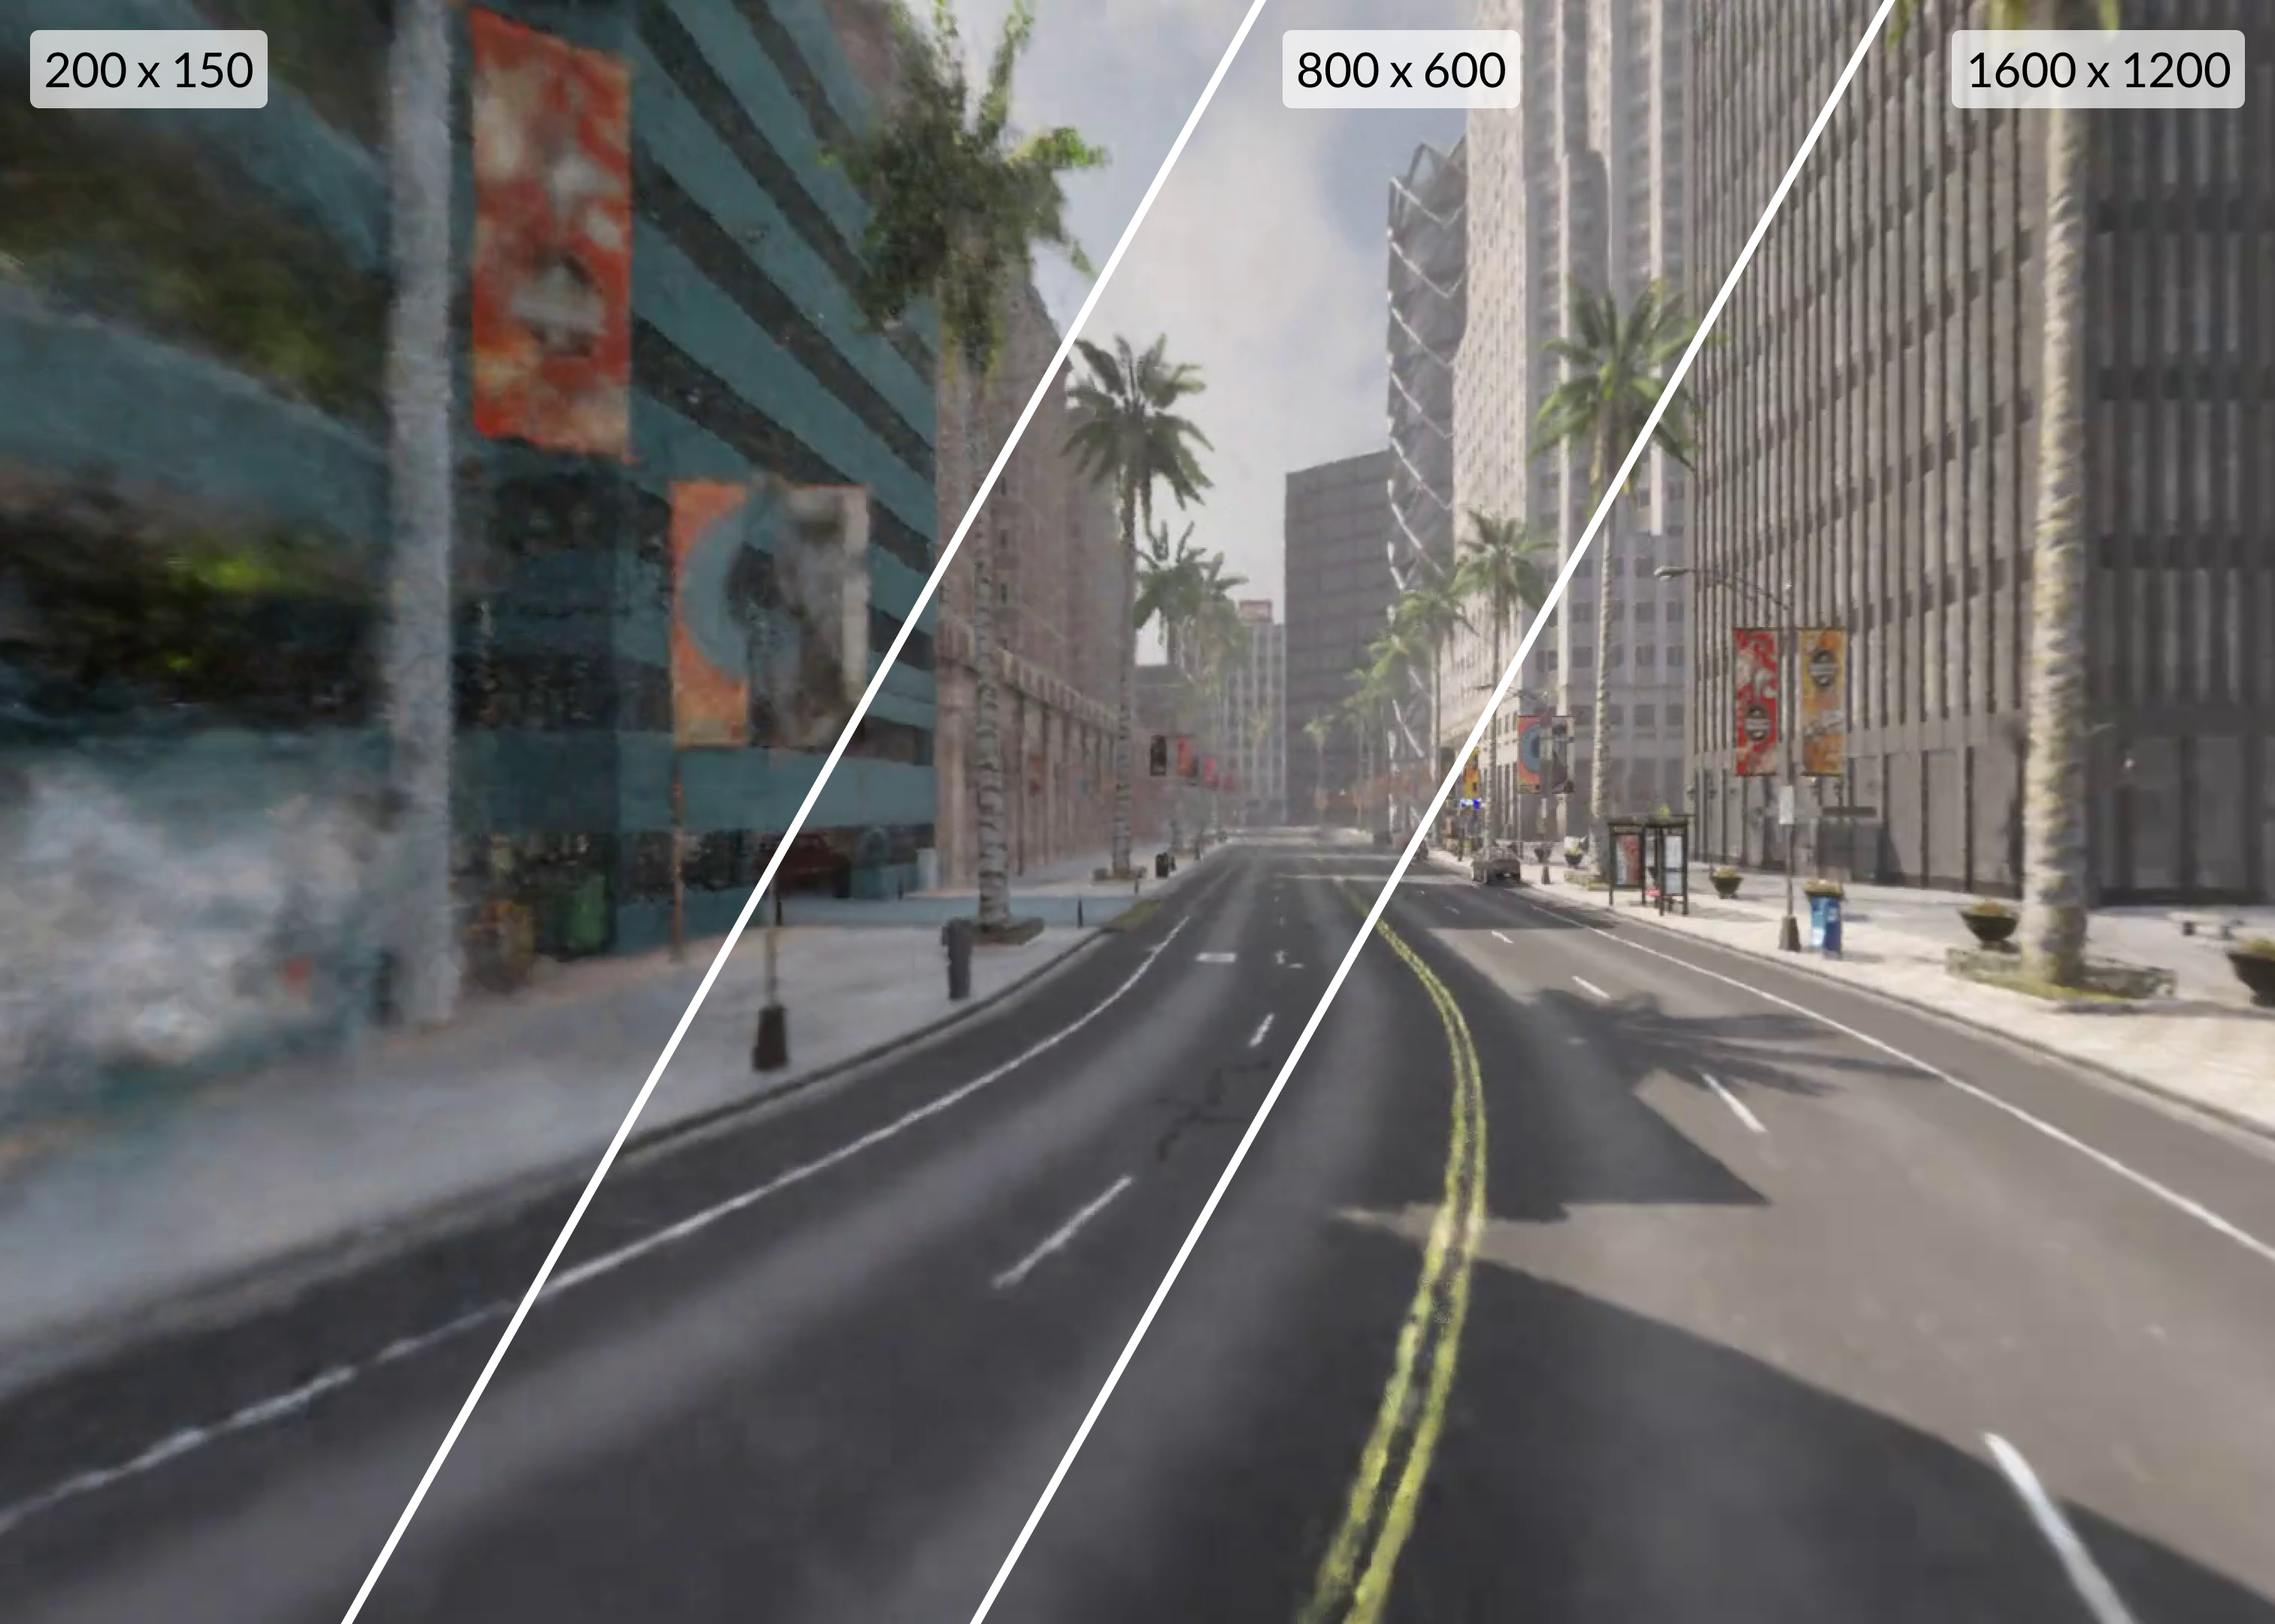
\includegraphics[width=1.0\textwidth]{figures/image-size-comparison.png}
    \caption{Comparison of frames rendered from models trained with training-data of different image resolution.}
    \label{fig:image-size-comparison}
\end{figure}

\subsection{Vehicle speed}
In order to test how much the vehicle speed contributes to the quality of data capture I performed 4 different experiments on vehicle speed.

\begin{table}[ht]
\centering
\caption{Results for exp\_speed-2}
\label{tab:exp_speed-2}
\begin{tabular}{|l|c|c|c|c|}
\hline
& description & psnr & ssim & lpips \\
\hline
0 & 0 & $\cellcolor{green} 24.061440$ & $\cellcolor{green} 0.775393$ & $\cellcolor{green} 0.181360$ \\
\cline{1-5}
1 & 1 & 23.502066 & 0.755476 & 0.184455 \\
\cline{1-5}
2 & 2 & 23.411259 & 0.742473 & 0.189968 \\
\cline{1-5}
3 & 3 & $\cellcolor{red} 22.717318$ & $\cellcolor{red} 0.713858$ & $\cellcolor{red} 0.200099$ \\
\cline{1-5}
\end{tabular}
\end{table}

\subsection{Combined baseline}
% I think this should be moved to method
From the experiments above, I combined the best configurations of the best results. The combined baseline consisted of:

\begin{itemize}
    \item Two forward-facing RGB-cameras, counterrotated with $-10^\circ$- and $10^\circ$ yaw.
    \item One lap. % Add a explanation of why I chose one lap, which yields the worst results.
    \item Image capture every second tick
    \item Image size of (400, 300)
    \item Vehicle speed that's 50\% slower than the current speed limit.
\end{itemize}

\begin{table}[ht]
\centering
\caption{Results for exp\_combined\_baseline\_2-0}
\label{tab:exp_combined_baseline_2-0}
\begin{tabular}{|l|c|c|c|c|}
\hline
 & description & psnr & ssim & lpips \\
\hline
0 & 0 & 24.197817 & 0.766733 & 0.168807 \\
\cline{1-5}
\end{tabular}
\end{table}


\section{Adding noise}
\begin{comment}
Information about GNSS-error
https://junipersys.com/support/article/6614#:~:text=Just%20as%20a%20general%20observation,to%202%20m%20vertical%20accuracy.
\end{comment}

\begin{table}[ht]
\centering
\caption{Results for exp\_gaussian\_noise-2}
\label{tab:exp_gaussian_noise-2}
\begin{tabular}{|l|c|c|c|c|}
\toprule
 & description & psnr & ssim & lpips \\
\midrule
0 & 0 & $\cellcolor{green} 23.609739$ & $\cellcolor{green} 0.754924$ & $\cellcolor{green} 0.171715$ \\
\cline{1-5}
1 & 1 & 18.499672 & 0.486572 & 0.240731 \\
\cline{1-5}
2 & 2 & 16.924616 & 0.407149 & 0.297813 \\
\cline{1-5}
3 & 3 & $\cellcolor{red} 16.297756$ & $\cellcolor{red} 0.384611$ & $\cellcolor{red} 0.553038$ \\
\cline{1-5}
\bottomrule
\end{tabular}
\end{table}


\begin{table}[ht]
\centering
\caption{Results for exp\_gaussian\_noise\_no\_optimizer-2}
\label{tab:exp_gaussian_noise_no_optimizer-2}
\begin{tabular}{|l|c|c|c|c|}
\toprule
 & description & psnr & ssim & lpips \\
\midrule
0 & 0 & $\cellcolor{green} 23.913687$ & $\cellcolor{green} 0.771429$ & $\cellcolor{green} 0.166504$ \\
\cline{1-5}
1 & 1 & 19.446724 & 0.503864 & 0.414767 \\
\cline{1-5}
2 & 2 & 18.099987 & 0.438293 & 0.482692 \\
\cline{1-5}
3 & 3 & $\cellcolor{red} 15.964767$ & $\cellcolor{red} 0.381585$ & $\cellcolor{red} 0.590534$ \\
\cline{1-5}
\bottomrule
\end{tabular}
\end{table}

\begin{table}
\centering
\caption{Results for exp\_gaussian\_noise\_shorter\_segments-2}
\label{tab:exp_gaussian_noise_shorter_segments-2}
\begin{tabular}{|l|c|c|c|c|}
\toprule
& description & psnr & ssim & lpips \\
\midrule
0 & 0 & $\cellcolor{green} 24.795582$ & $\cellcolor{green} 0.833400$ & $\cellcolor{red} 0.102616$ \\
\cline{1-5}
1 & 1 & 22.735580 & 0.725762 & 0.121869 \\
\cline{1-5}
2 & 2 & 20.316860 & 0.597075 & 0.152559 \\
\cline{1-5}
3 & 3 & $\cellcolor{red} 19.765114$ & $\cellcolor{red} 0.550024$ & $\cellcolor{green} 0.172539$ \\
\cline{1-5}
\bottomrule
\end{tabular}
\end{table}

As seen in \autoref{tab:exp_gaussian_noise_shorter_segments-2} the metrics show better results than \autoref{tab:exp_gaussian_noise-2}. The noise seems to have a greater impact on the resulting scene, the larger the scene is. 


\section{COLMAP vs. Absolute poses}

The results are almost equal. Need to look at the qualitative results.

\begin{table}[ht]
\centering
\caption{Results for experiments}
\label{tab:experiment_results}
\begin{tabular}{|l|c|c|c|}
\hline
\textbf{Experiment Name} & \textbf{PSNR} & \textbf{SSIM} & \textbf{LPIPS} \\ \hline
exp\_combined\_baseline\_2-0 & $\cellcolor{green} 24.197817$ & $\cellcolor{green} 0.766733$ & $\cellcolor{red} 0.168807$ \\ \hline
data-images-exp\_combined\_baseline\_2\_colmap & $\cellcolor{red} 24.18618$ & $\cellcolor{red} 0.758549$ & $\cellcolor{green} 0.159935$ \\ \hline
\end{tabular}
\end{table}

\section{Different models}
Nerfstudio have implemented multiple well-known NeRF-models. In this experiment I'd like to see if changing the models would have any impact on the output.



\section{Block NeRF}

By splitting the scene into smaller segments, the combined scene generates better results than when the entire scene is trained within a single NeRF. The average PSNR is 24.4746 - which is 0.2768 better than the entire scene in one. Block NeRF's high quality will sustain large scenes, where a single NeRF will start deteriorating as the scene size increases.

\begin{table}[ht]
\centering
\begin{tabular}{|l|c|c|c|c|}
\hline
& description & psnr & ssim & lpips \\
\hline
0 & 0 & 24.960262 & 0.815270 & 0.161623 \\
\cline{1-5}
1 & 1 & 25.660400 & 0.824085 & 0.164296 \\
\cline{1-5}
2 & 2 & 23.914209 & 0.755183 & 0.194245 \\
\cline{1-5}
3 & 3 & 23.363695 & 0.764547 & 0.216242 \\
\cline{1-5}
\hline
\end{tabular}
\caption{Results for exp\_combined\_baseline\_block\_nerf}
\label{tab:exp_combined_baseline_block_nerf}
\end{table}


\begin{table}
\centering
\caption{Results for exp\_block\_nerf\_long\_path\_2-block\_10}
\label{tab:exp_block_nerf_long_path_2-block_10}
\begin{tabular}{|l|c|c|c|c|}
\toprule
 & description & psnr & ssim & lpips \\
\midrule
0 & 0 & 25.047100 & 0.826931 & 0.138852 \\
\cline{1-5}
1 & 1 & $\cellcolor{green} 25.703838$ & 0.831167 & 0.156331 \\
\cline{1-5}
2 & 2 & 24.924395 & 0.830144 & 0.149870 \\
\cline{1-5}
3 & 3 & $\cellcolor{red} 22.726223$ & $\cellcolor{red} 0.713277$ & $\cellcolor{red} 0.207025$ \\
\cline{1-5}
4 & 4 & 25.468483 & 0.837942 & $\cellcolor{green} 0.131815$ \\
\cline{1-5}
5 & 5 & 25.670006 & $\cellcolor{green} 0.841962$ & 0.147232 \\
\cline{1-5}
6 & 6 & 25.661350 & 0.820813 & 0.163685 \\
\cline{1-5}
7 & 7 & 25.070913 & 0.777114 & 0.154277 \\
\cline{1-5}
8 & 8 & 24.803871 & 0.814633 & 0.154028 \\
\cline{1-5}
9 & 9 & 23.693977 & 0.753770 & 0.185557 \\
\cline{1-5}
10 & 10 & 23.936722 & 0.757462 & 0.179283 \\
\cline{1-5}
11 & 11 & 24.584238 & 0.807874 & 0.144022 \\
\cline{1-5}
\bottomrule
\end{tabular}
\end{table}


\begin{table}
\centering
\caption{Results for exp\_block\_nerf\_long\_path\_no\_blocks-0 compared to the results of exp\_block\_nerf\_long\_path\_2-block\_10}
\label{tab:exp_block_nerf_long_path_no_blocks-0}
\begin{tabular}{|l|c|c|c|c|}
\toprule
  & description & psnr & ssim & lpips \\
\midrule
0 & 0 & $\cellcolor{red} 22.515461$ & $\cellcolor{red} 0.654036$ & $\cellcolor{red} 0.424356$ \\
\cline{1-5}
1 & Average of 12 block NeRF & $\cellcolor{green} 24.774259$ & $\cellcolor{green} 0.801090$ & $\cellcolor{green} 0.159331$ \\
\cline{1-5}
\bottomrule
\end{tabular}
\end{table}

\begin{figure}[!h]
    \centering
    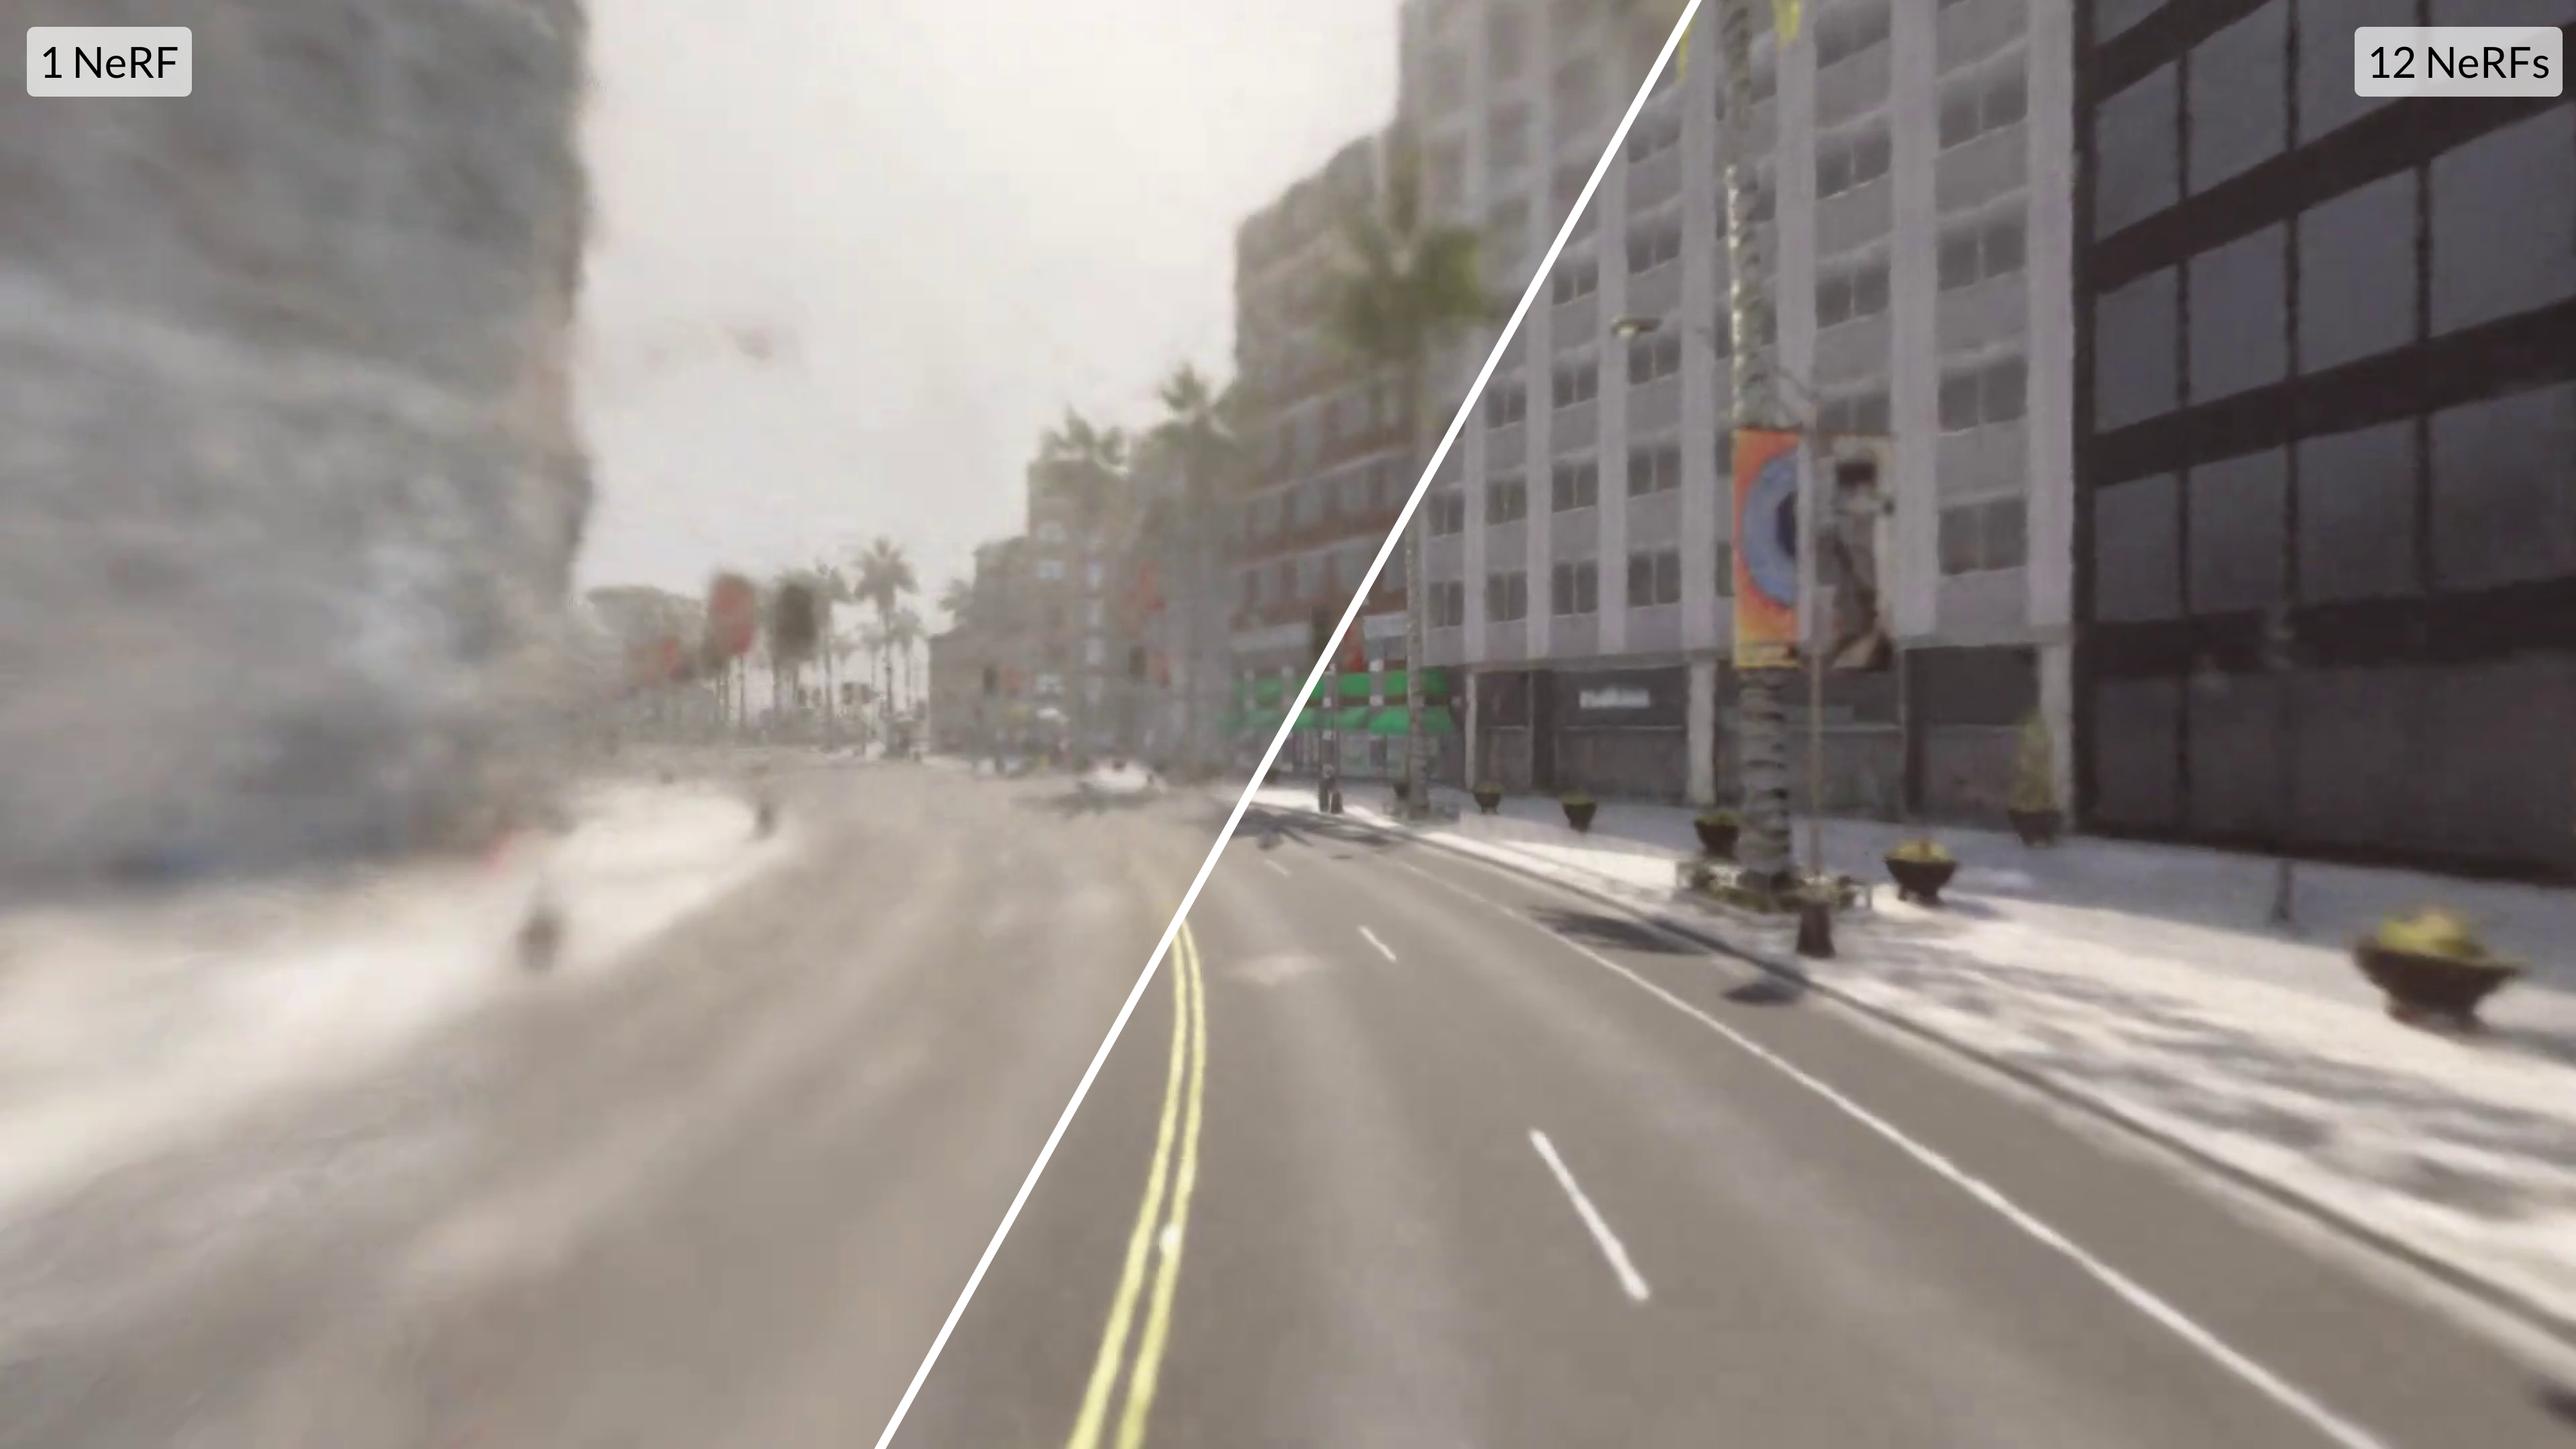
\includegraphics[width=1.0\textwidth]{figures/block-nerf-comparison.png}
    \caption{Comparison of two renders from models who have been trained on the same data. Left) One NeRF trained on all data, Right) 12 NeRFs trained on equally spaced segments.}
    \label{fig:block-nerf-comparison}
\end{figure}

\begin{figure}[!h]
    \centering
    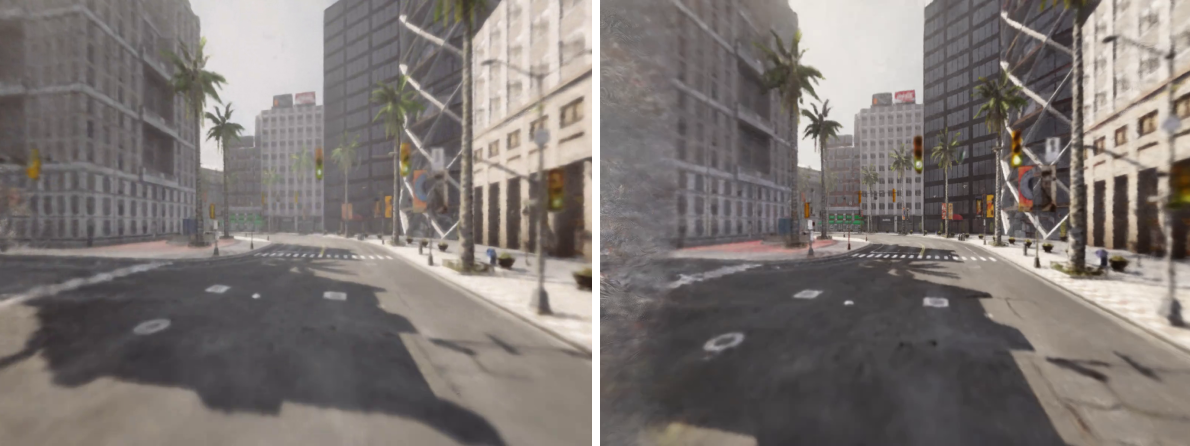
\includegraphics[width=1.0\textwidth]{figures/block-nerf-frame-comparison.png}
    \caption{Comparison of two consecutive frames of a single render on a 12 block NeRF. The first frame (left) is the last frame rendered by block number 1. The second frame (right) is the first frame rendered by block number 2. The details of the scenery in the second frame is clearly better than the first, which is expected as block number 2 have been trained on close-up images of the scene. This difference could be mitigated by looking into image merging techniques such as inverse distance weighing.}
    \label{fig:block-nerf-frame-comparison}
\end{figure}